\documentclass{replab}
\usepackage{lipsum}
\usepackage{float}
\usepackage{biblatex}

% --- Información del documento ---
\title{Laboratorio de Electrónica}
\author{Alarcón Pérez Bruno}

\date{14 de abril de 2026}
\subtitle={Práctica 2: INSTRUMENTACIÓN Y SEÑALES}
\email={\href{mailto:bruno_alarcon@ciencias.unam.mx}{\color{principaluno}\texttt{bruno\_alarcon@ciencias.unam.mx}}}
\subject={Laboratorio de Electrónica}

\setlength{\columnsep}{14pt}

% --- Archivo de bibliografía ---
\addbibresource{repbib.bib}

% --- Inicio del documento ---
\begin{document}
	
	\pagestyle{fancy}
	\unspacedoperators
	
% --- Título ---
	\twocolumn[
		\begin{center}
			\maketitle
			
			\smallskip
		\end{center}
	]
	
% --- Cuerpo del reporte ---
	
	\section{Tipos de Instrumentos}
	A lo largo de la práctica se trabajó con dos tipos de instrumentos, aquellos que generan y dan algun tipo de señal y aquellos que reciben dichas
	señales. Por supuesto, existen algunos los cuales son de ambos tipos. Cada instrumento tiene sus propias características incluso diferenciándose
	por la marca o precio.\\

	Una de las razones por las que un instrumento podría no medir correctamente es el \textbf{Acoplamiento de Impedancias} (impedance bringing),
	el cual nos dice que la impedancia de entrada debe ser mucho mayor que la impedancia de salida, es decir, para que los intrumentos no sufran daños,
	aquellos que entregan señal deben tener menor impedancia con respecto a aquellos que reciben señal.\\
	Un gran ejemplo puesto a prueba fue conectar una bocina de $8 \Omega$ directamente al generador de funciones el cual tiene una impedancia de
	$50 \Omega$ a una frecuencia en el rango de audición humana, lo cual evidentemente nos generó un problema de acoplamiento de impedancias, lo cual se
	observó como una disminución de voltaje como una medida de protección del instrumento, además se escuchó una señal algo distorsionada.

		\subsection{Entregan señal}
		Aqui tenemos como ejemplo a la \textbf{Fuente DC}, el cual genera un voltaje constante. Cuenta con dos perillas, una para controlar el voltaje
		y otro para la corriente, dichos valores se muestran en una pantalla. Cuenta con tres terminales tipo banana, dos para positivo y negativo y otro
		entre estos que funciona como la tierra. Es recomendable antes de encender el generador, revisar que la perilla del voltaje este al mínimo y la
		de corriente al máximo.

		El \textbf{Generador de Funciones} genera una señal de voltaje alterno, es decir, que no es constante a diferencia de la Fuente DC.
		Podemos elegir la forma de la señal, ya sea senoidal, triangular o cuadrada, además, se puede ajustar su frecuencia. Funciona con terminales BNC.

		El \textbf{Generador del EGOS} es un instrumento que si bien no cuenta pantallas
		como gran parte de los demás instrumentos, sigue cumpliendo su papel como generador de hasta tres señales de voltaje AC con forma
		senoidal, teniendo perillas para controlar voltaje y frecuencia y otras opciones como el barrido y la fase que se explicarán más adelante.
		
		La \textbf{Fuente Simétrica} y el \textbf{Transformador} son similares a la Fuente DC y al Generador de Funciones, respectivamente, pero
		a diferencia de estos, ambos ofrecen, dependiendo de la manera en que se conecten los cables a estos; $\pm$ el voltaje nominal si un cable va al
		positivo y otro al negativo o $\pm$ el doble de este si uno de los cables va a la tierra del instrumento.
		
		\subsection{Reciben señal}
		Aquí se encuentran los instrumentos que ``miden'' las señales, pues son los que regresan valores como el voltaje, corriente e incluso frecuencia
		como se verá posteriormente.\\
		En primer lugar, tenemos como ejemplo al \textbf{Multímetro} que, como su nombre lo indica, nos permite medir diferentes parámetros
		como el voltaje y corriente tanto en DC como en AC (Voltaje RMS), resistencia, capacitancia, etc. El instrumento recibe la señal de
		otro que entrega señal y nos devuelve la medición del parámetro que queramos, en otras palabras, este instrumento nos sirve para
		\textit{medir cuantitativamente} una señal. Para ello, cuenta con terminales tipo banana que, dependiendo de lo que queramos medir,
		se utilizará una u otra, pero la conexión que no puede faltar es la de la terminal que sirve como referencia (tierra).\\

		Por otro lado, el \textbf{Osciloscopio} nos permite visualizar graficamente una o dos señales de voltaje, estas se pueden ver en una
		cuadrícula de voltaje contra tiempo donde la escala es ajustable, en otras palabras, nos permite \textit{medir cualitativamente} una señal, es decir,
		su forma, si tiene ``ruido'' o mejor dicho que tanto ``ruido'' tiene, etc.\\
		Este instrumento cuenta con muchas opciones, entre ellas permite recibir dos señales mediante dos terminales BNC de dos fuentes distintas
		y visualizarlas sobre una misma gráfica, mover dichas señales de posición vertical y horizontal, ajustar la escala temporal y de voltaje,
		un cursor que nos permite medir dentro del instrumento que, por lo tanto, también permite \textit{medir cuantitativamente} una señal cuando
		se leen los valores, y otra muy importante, la opción ``math'' que nos habilita, por ejemplo, la Transformada de Fourier. Podemos ver el osciloscopio
		de la marca Tektronix en la Figura \ref{fig:osciloscopio}.\\

		De momento puede parecer que el osciloscopio es muy superior al multímetro pues puede medir cuantitativamente y cualitativamente, sin embargo, 
		sí hay diferencia entre medir con el multímetro o con el osciloscopio, pues por ejemplo, el osciloscopio no puede medir corriente o resistencia a
		diferencia del multímetro, además, este último es mucho más seguro debido a que puede soportar mayor voltaje. Por ejemplo, si queremos medir
		la linea, ya sabemos que esta es una AC con forma senoidal, por lo que solo interesaría medir con el osciloscopio si se requiere ver si hay ruidos en ella.

		\begin{figure}[ht]
			\centering
			\begin{subfigure}[b]{0.48\columnwidth}
				\centering
				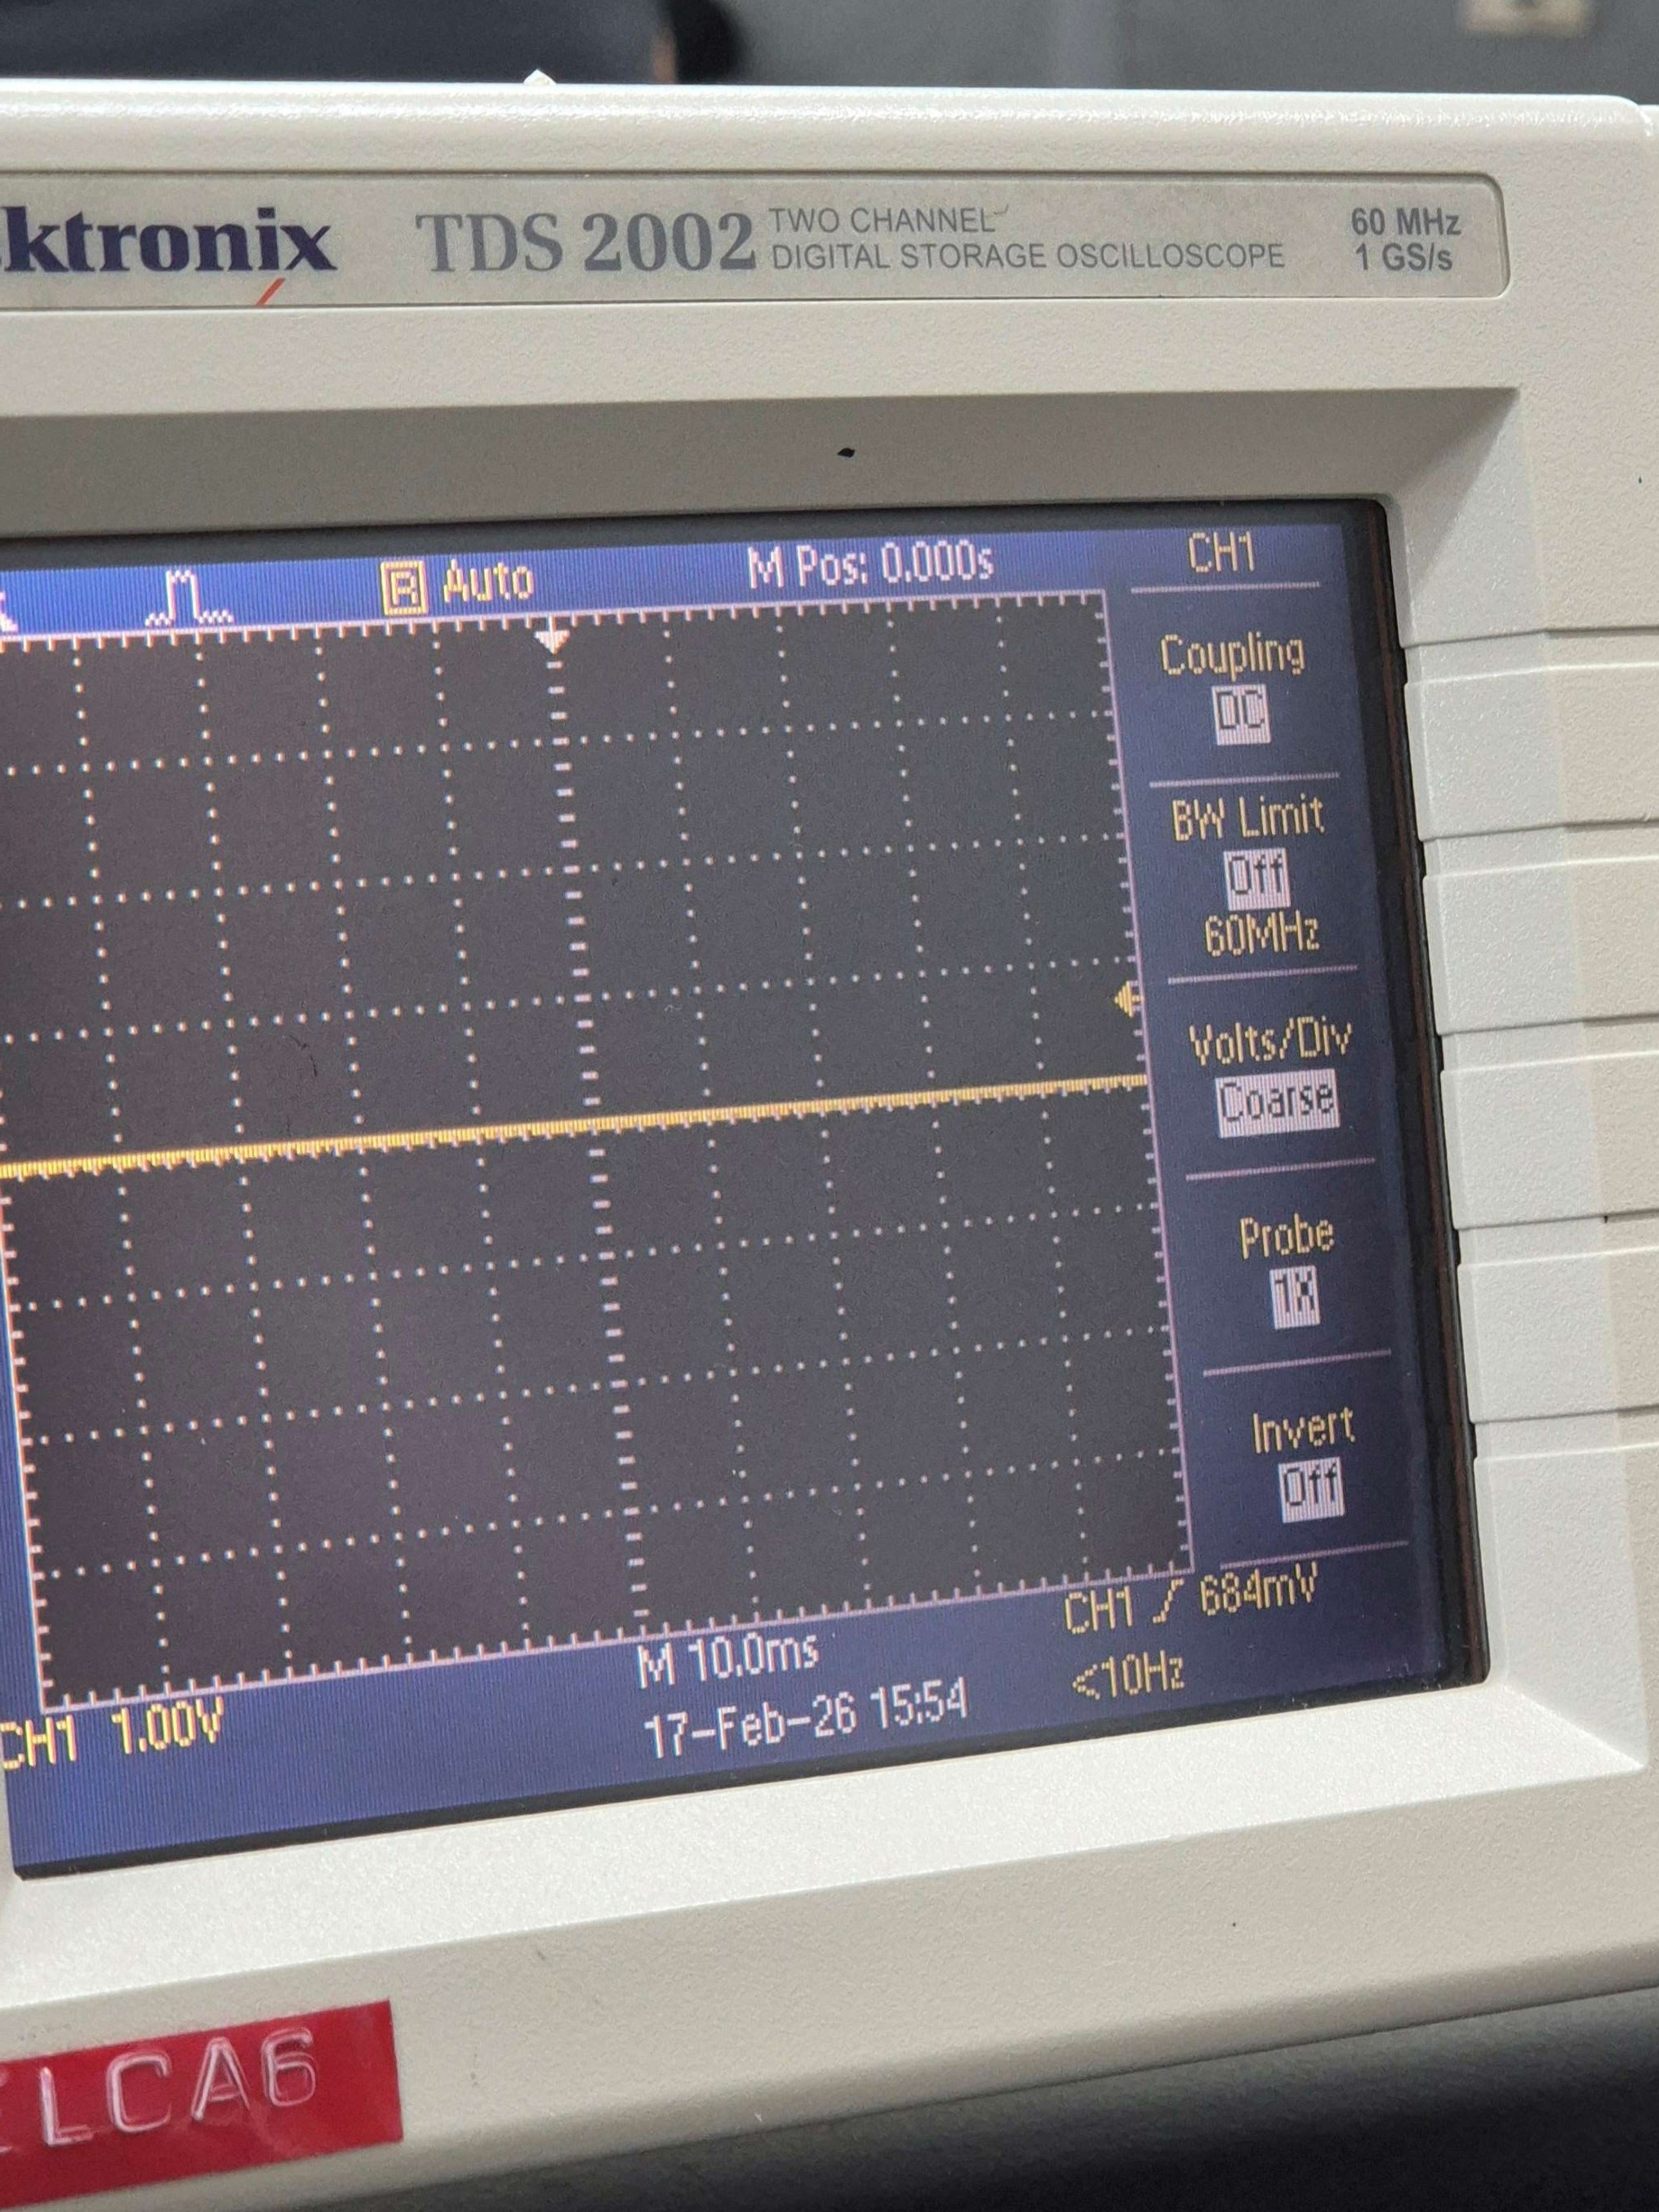
\includegraphics[width=\linewidth, keepaspectratio]{imagenes/osciloscopio1.jpg}
			\end{subfigure}
			\hfill
			\begin{subfigure}[b]{0.48\columnwidth}
				\centering
				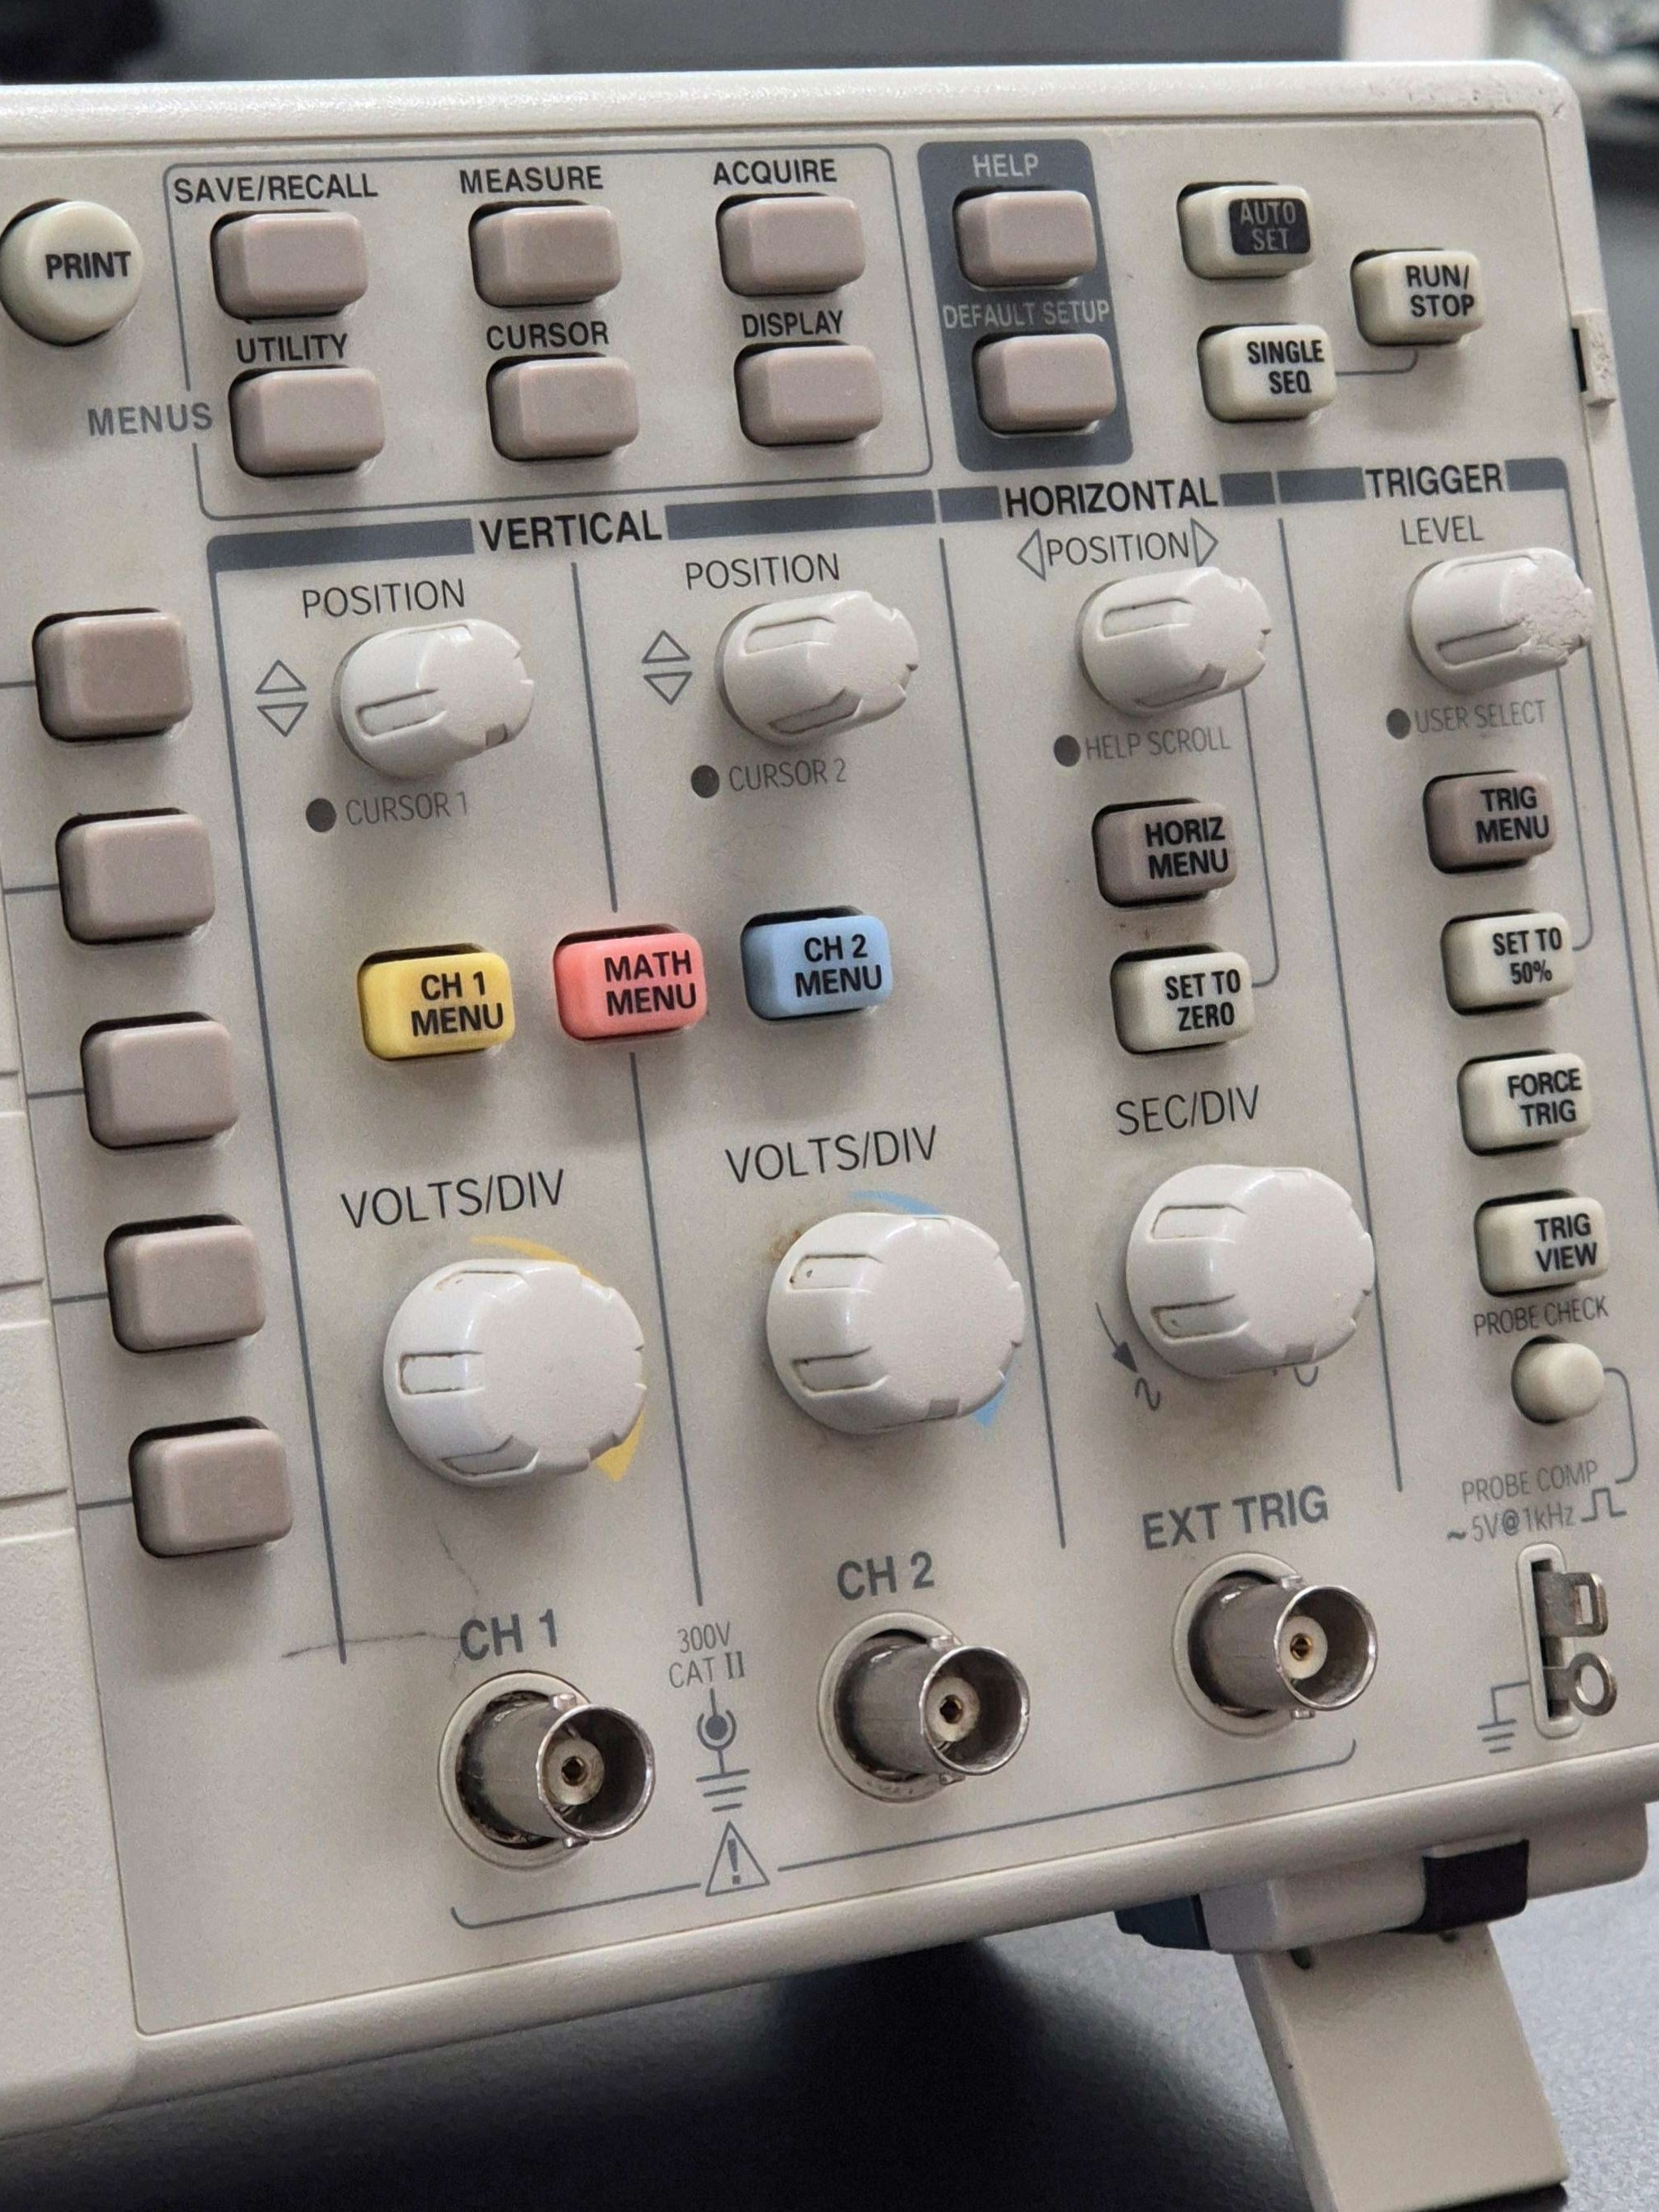
\includegraphics[width=\linewidth, keepaspectratio]{imagenes/osciloscopio2.jpg}
			\end{subfigure}
			\caption{Osciloscopio}
			\label{fig:osciloscopio}
		\end{figure}

		El \textbf{Sumador del EGOS} es un buen ejemplo de un instrumento que recibe y entrega señal, pues por una parte, tiene 3 entradas BNC las cuales
		permiten conectar 3 señales completamente distintas a este insrumento y, mediante una única salida BNC, este instrumento ``suma'' las señales y las
		manda por este canal de salida hacia otro instrumento como el osciloscopio.

	\section{Transformada de Fourier}
	La Transformada de Fourier es una herramienta que nos transforma una funcion periódica de un cierto espacio al espacio de
	frecuencias. El osciloscopio cuenta con esta función en el botón de ``math'' y en la opcion ``FFT (Fast Fourier Transform)'', al presionar
	dichas opciones la pantalla del osciloscopio cambia al espacio de frecuencias donde el eje temporal ahora es el eje de frecuencias $(Hz)$
	y el eje de voltaje ahora es el eje de decibeles y aparece en escala logarítmica para que a diferentes voltajes las frecuencias se puedan
	visualizar correctamente.
	% Derrame espectral
		
		\subsection{FFT Senoidal, Cuadrada y Triangular}
		Se montó un pequeño circuito como el mostrado en la Figura \ref{fig:triangular} en el que se generaron, con el generador de funciones a $3.5 V_{RMS}$
		y $1 kHz$, tres formas de onda distintas y se observaron em el osciloscopio conectado a la vez con el multímetro.\\
		
		Para el primer caso, se generó una onda senoidal en el que se observó en la FFT un solo pico que coincide con la frecuencia seleccionada en el generador.
		En cuanto a los siguientes casos, pasamos a una onda triangular y posteriormente a una onda cuadrada, en la que se observó un aumento en la amplitud y
		en ambas y en la FFT se logró ver la frecuencia fundamental y los armónicos, es decir, más picos de frecuencia para ambos en la FFT. Cabe destacar que,
		en la onda triangular, los armónicos cayeron más rápido que en la cuadrada.

		Los valores obtenidos con el multímetro se encuentran en la Tabla \ref{tab:triangular} en el Apéndice \ref{apx:1}, en la que podemos notar el aumento
		de amplitud anteriormente mencionado, así como que, dado que la señal es de corriente alterna, las mediciones en DC tuvieron mucha variación.

		\begin{figure}[ht]
			\centering
			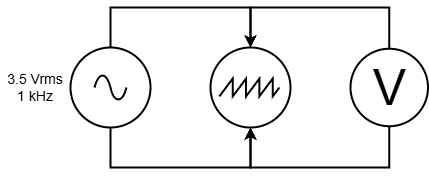
\includegraphics[width=0.40\textwidth]{imagenes/senoidal.drawio.png}
			\caption{Montaje del circuito para observar y medir diferentes formas de onda.}
			\label{fig:triangular}
		\end{figure}

		\subsection{EGOS Generador y Sumador}
		Para poner aun más a prueba la FFT del Osciloscopio y el EGOS (Estación Generadora y Operador de Señales), realizamos cuatro casos de suma de dos señales
		de voltaje con forma senoidal a partir de dos salidas del Generador del EGOS, las cuales se conectaron al Sumador del EGOS para luego conectar su salida
		al Osciloscopio.

		\begin{itemize}
			\item Para el primer caso, ambas señales tuvieron la misma frecuencia y amplitud. En el osciloscopio se observó el fenómeno de \textit{batimiento}
			pues la amplitud de la señal resultante era variable y llegaba hasta el doble de la amplitud de cada señal, inclusó se apreció muy bien la envolvente
			de esta. Por otro lado, en la FFT se observó un solo pico que, al hacerle ``zoom'', fue más evidente observar que se trataba de dos picos de la misma
			altura pero muy juntos, es decir, que efectivamente estabamos sumando dos frecuencias distintas pero casi idénticas, por ello el batimiento.
			Observar Figura \ref{fig:caso1}
			\begin{figure}[ht]
				\centering
				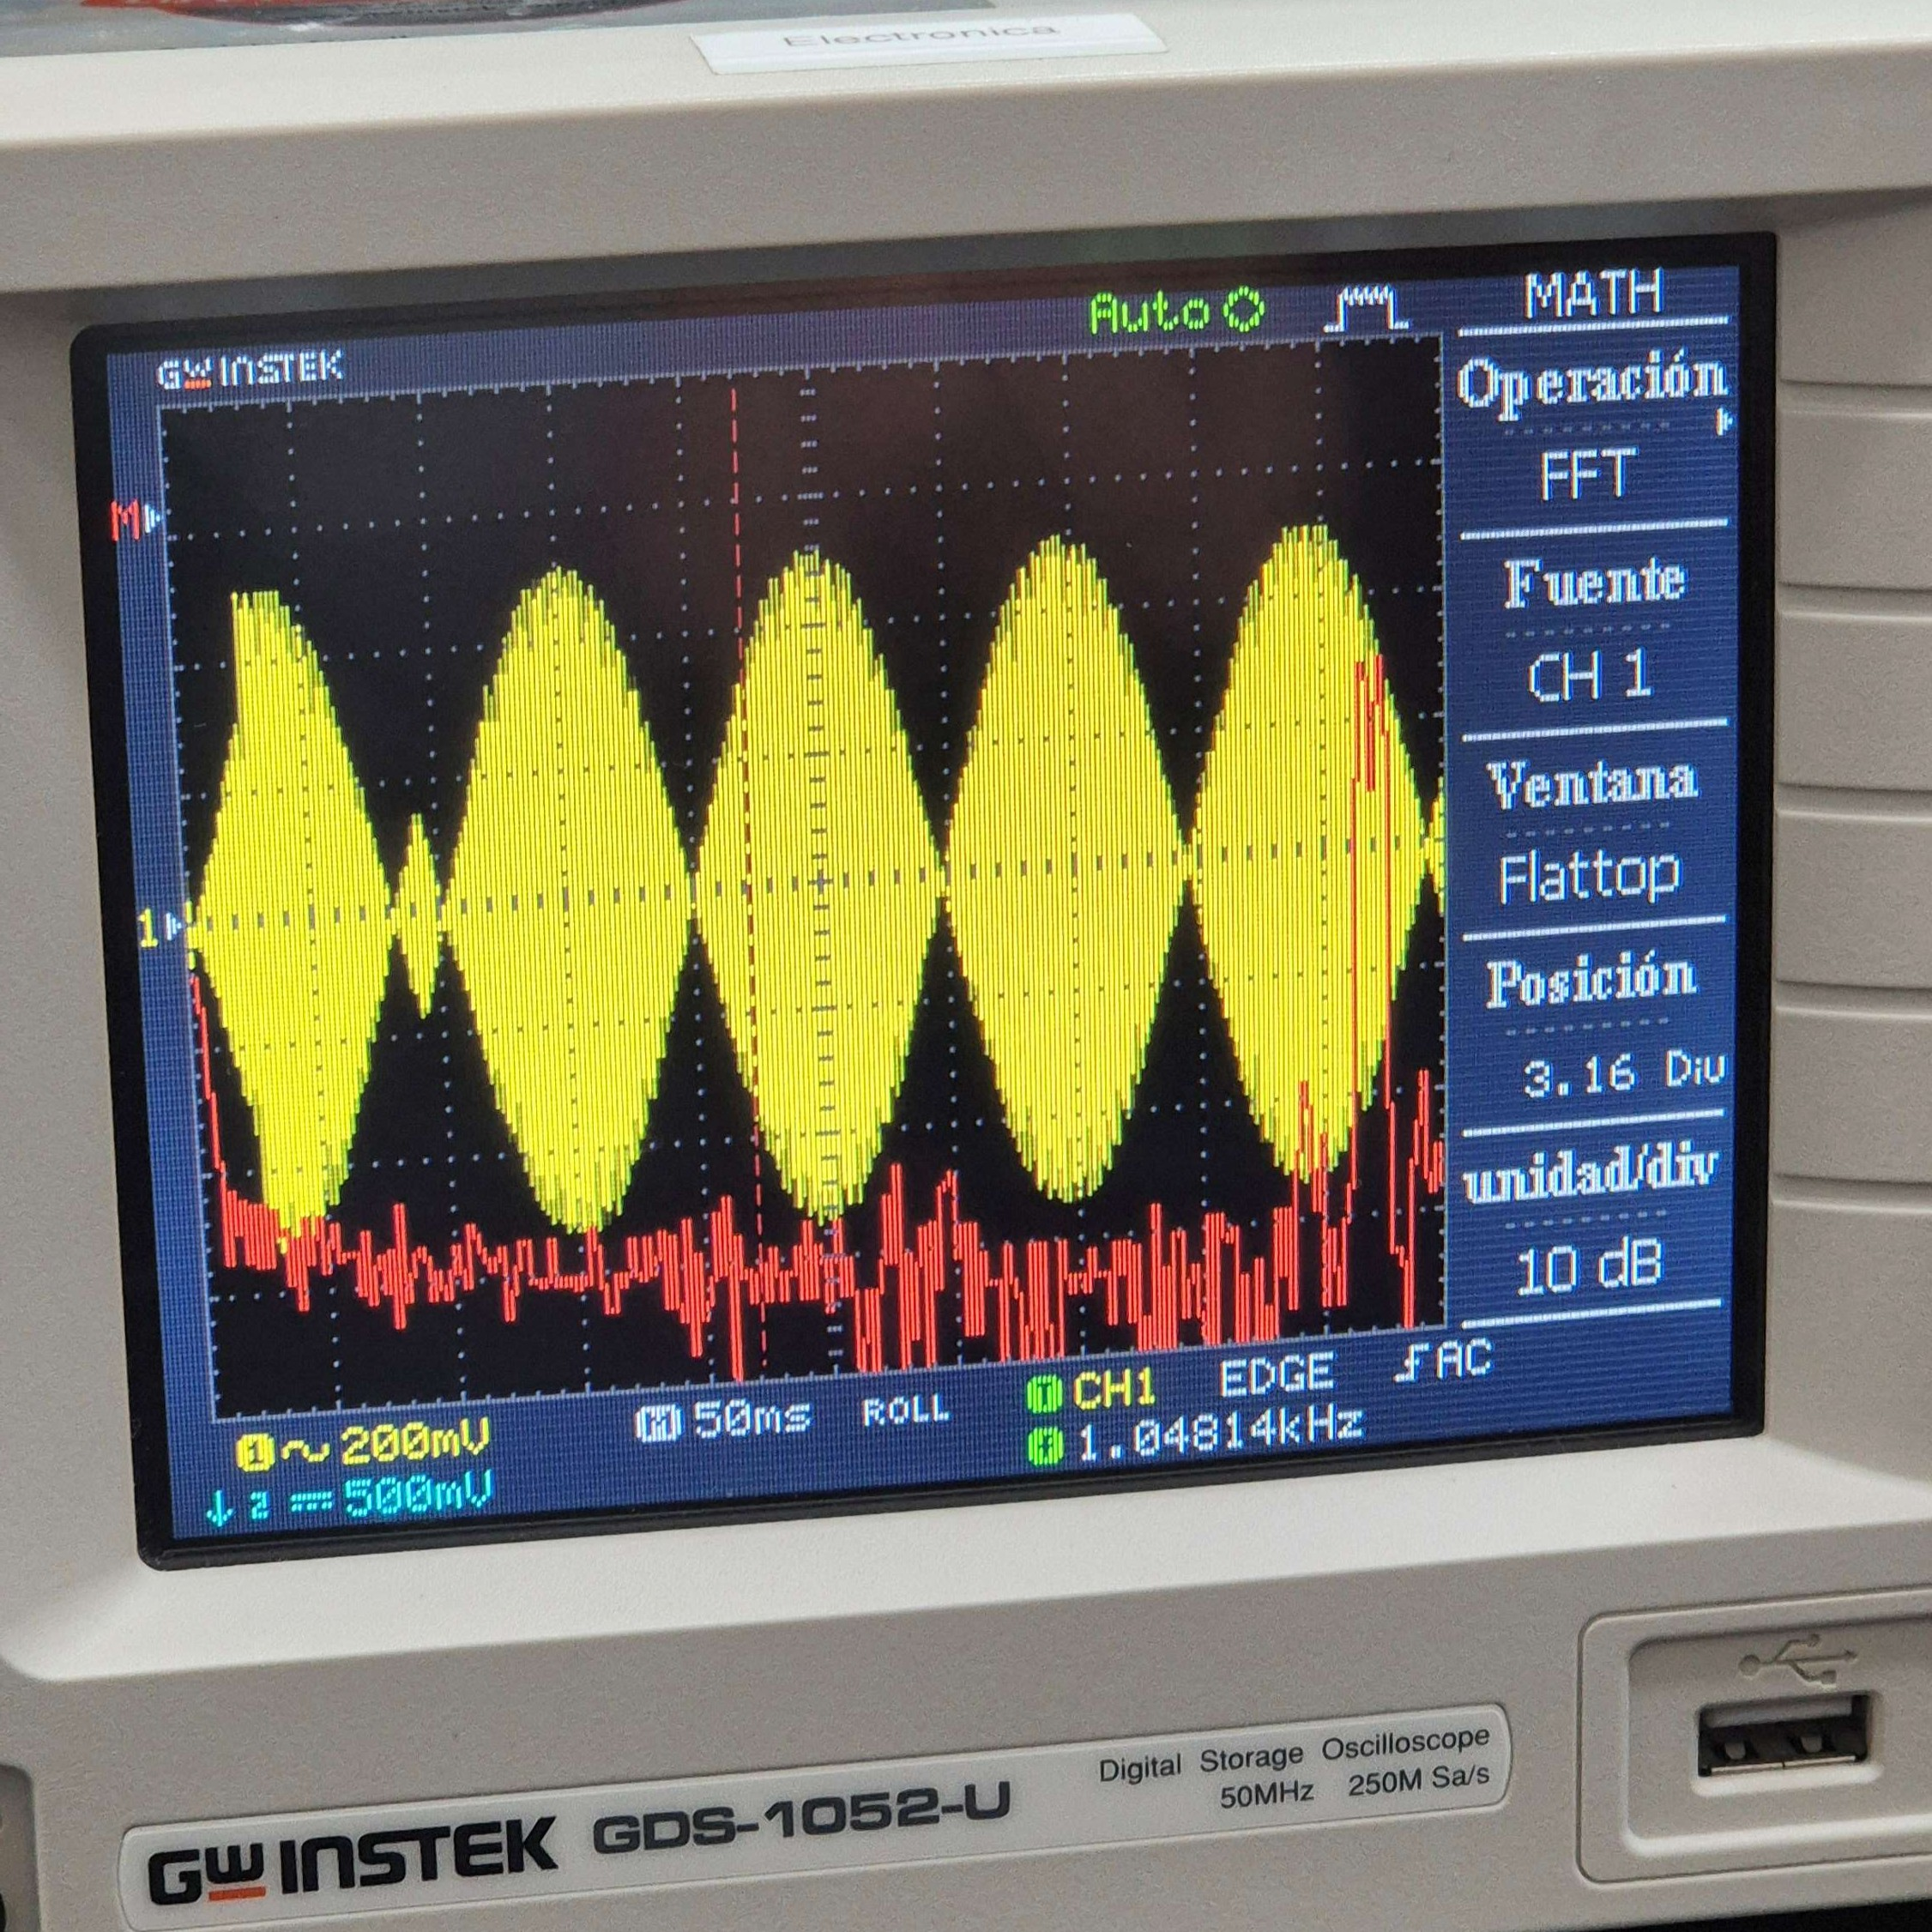
\includegraphics[width=0.35\textwidth]{imagenes/caso1.jpg}
				\caption{Caso 1: Frecuencias y amplitudes iguales.}
				\label{fig:caso1}
			\end{figure}
			\item Para el siguiente caso, se mantuvieron las frecuencias ``iguales'' pero las amplitudes fueron distintas, por lo que en el osciloscopio se mostró
			una señal similar a la anterior pero que en este caso no hubo interferencia completamente destructiva, es decir, que los mínimos quedaron ``levantados''
			de modo que la onda no desapareció competamente en ningún momento. En cuanto a la FFT, se observaron dos picos ``superpuestos'' pero con diferentes
			alturas, es decir que efectivamente sumamos la ``misma'' frecuencia pero a amplitudes distintas. Observar Figura \ref{fig:caso2}
			\begin{figure}[ht]
				\centering
				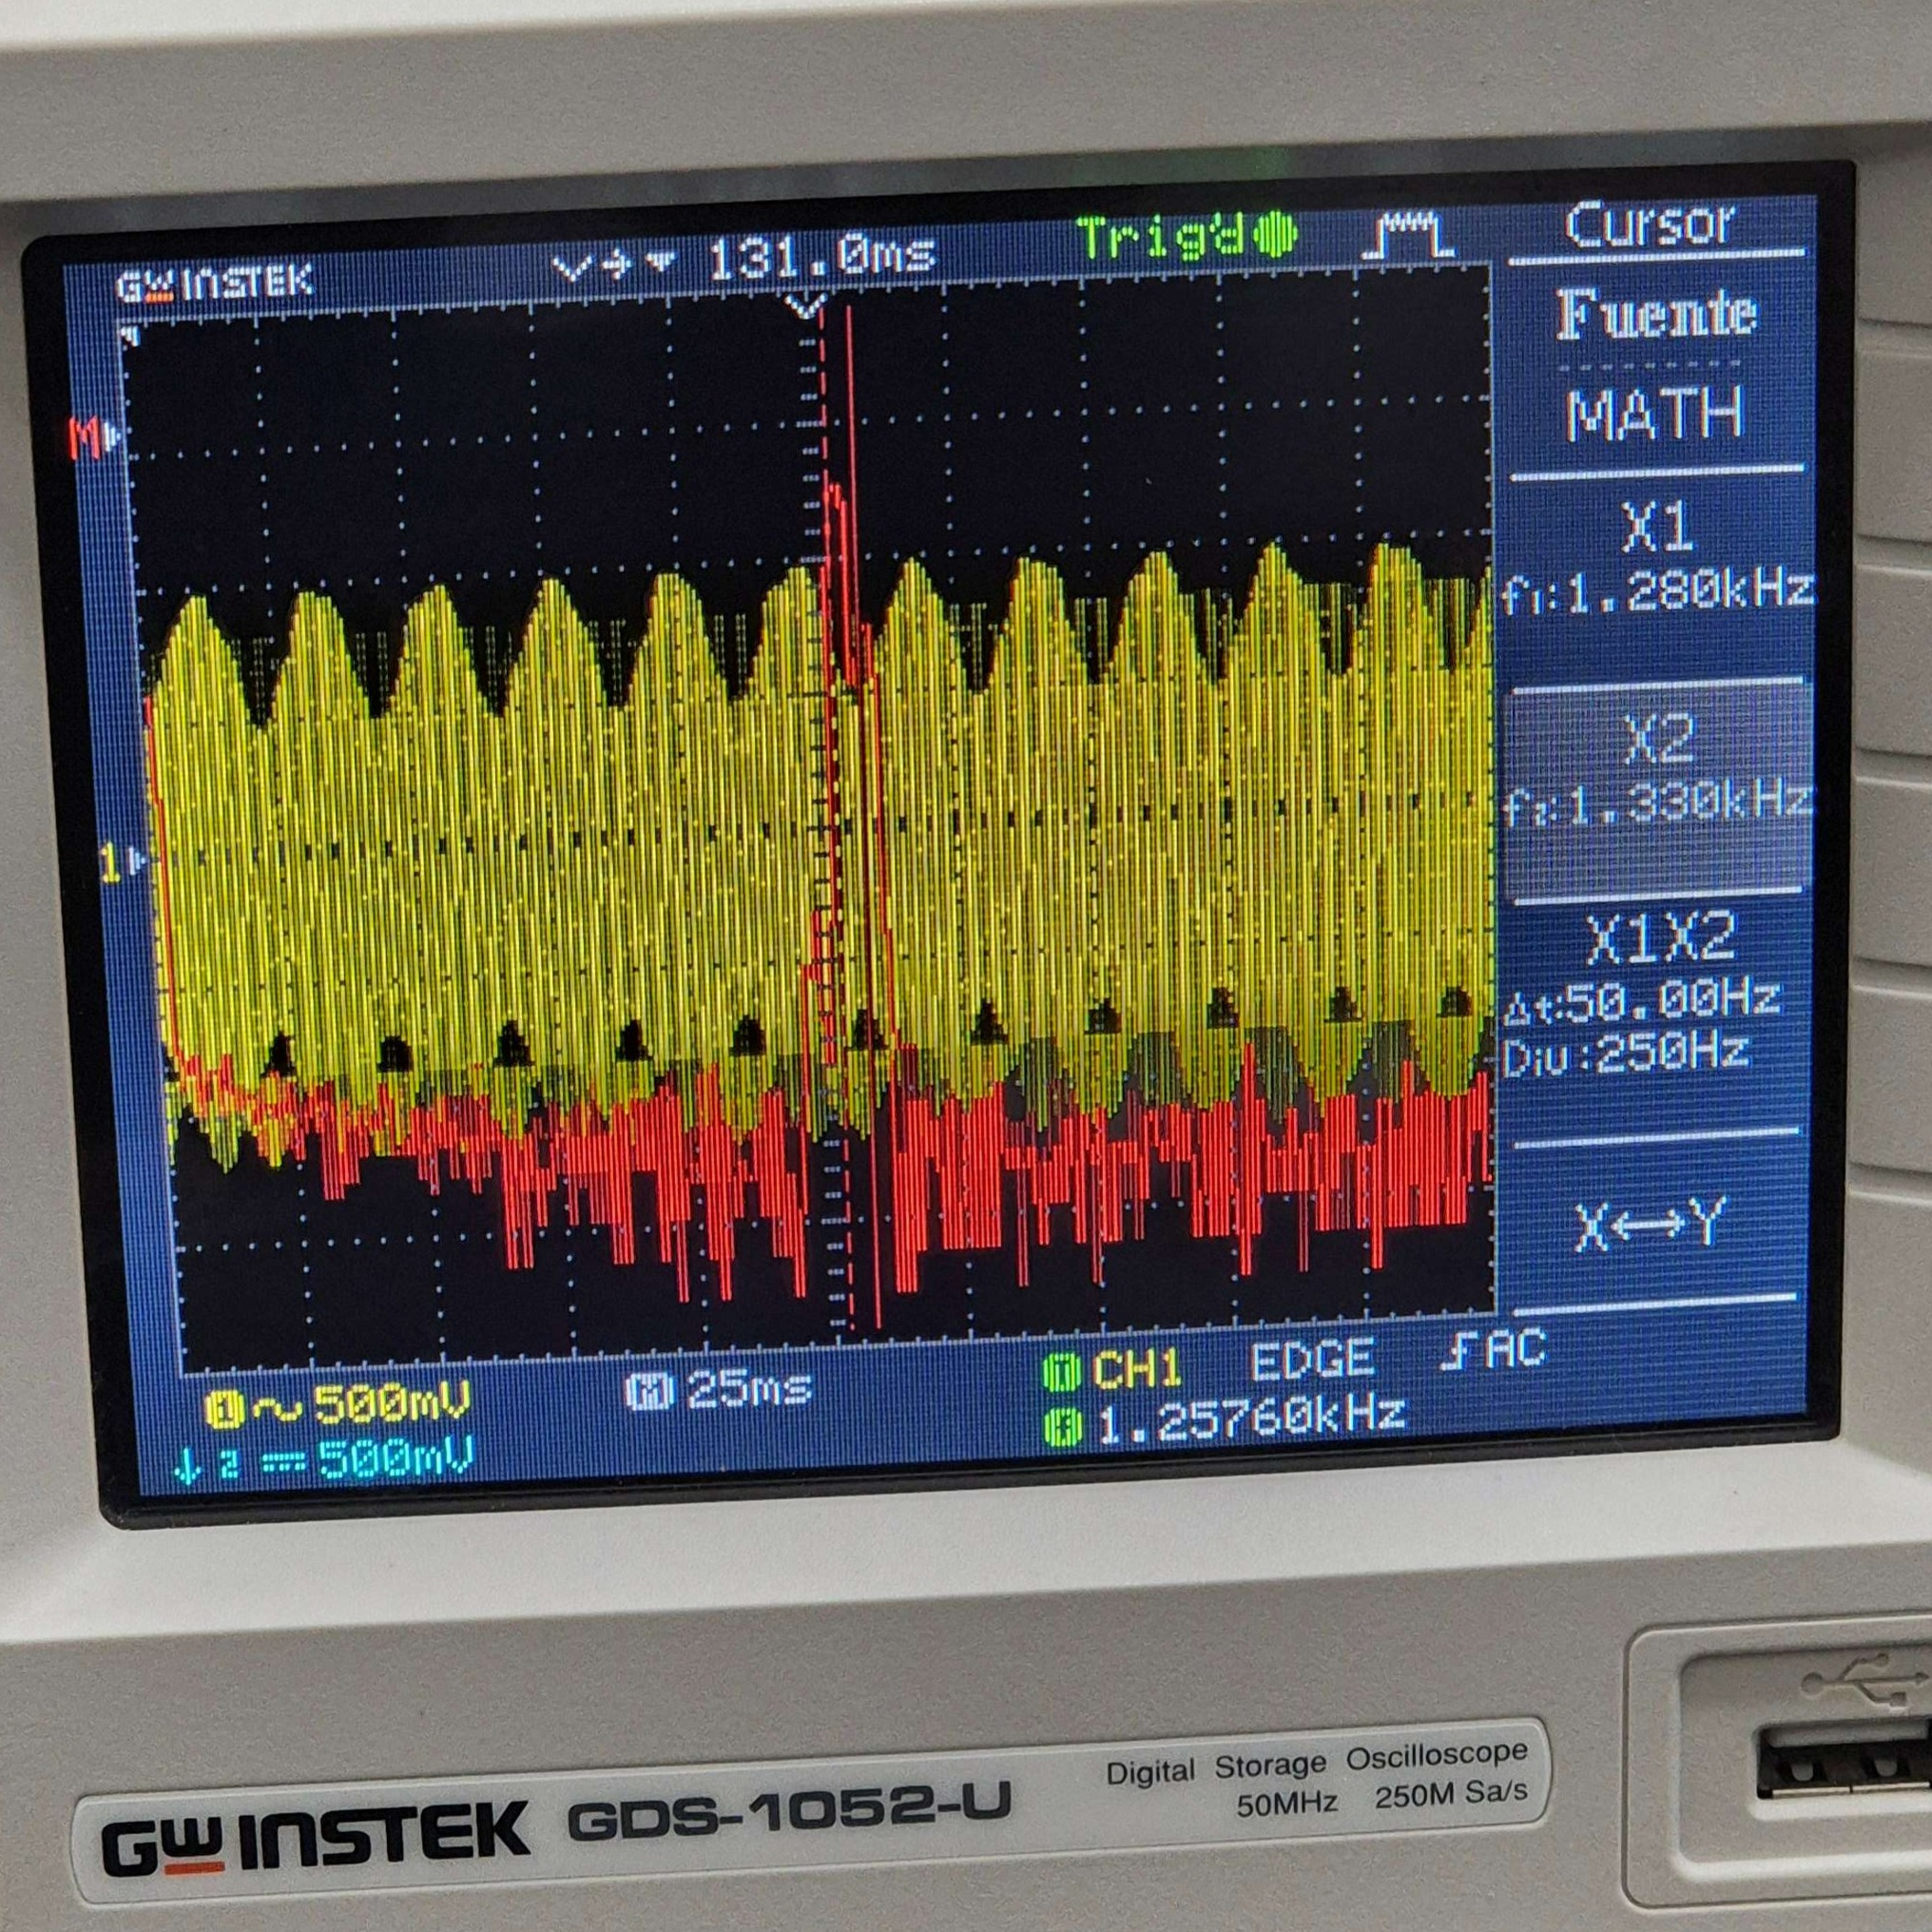
\includegraphics[width=0.35\textwidth]{imagenes/caso2.jpg}
				\caption{Caso 2: Frecuencias iguales amplitudes distintas.}
				\label{fig:caso2}
			\end{figure}
			\item Para el tercer caso, regresamos a tener las mismas amplitudes pero esta vez a diferentes frecuencias, por lo que en el osciloscopio se observó
			una señal compuesta donde la señal de mayor frecuencia se ``montó'' a la señal de menor frecuencia, en otras palabras, la señal de menor frecuencia
			estaba formada por otra señal con mayor frecuencia. En la FFT se logró observar dos picos con la misma altura pero esta vez más separados
			horizontalmente, es decir, la señal resultante es producto de señales con diferentes frecuencias y mismas amplitudes. Observar Figura \ref{fig:caso3}
			\begin{figure}[ht]
				\centering
				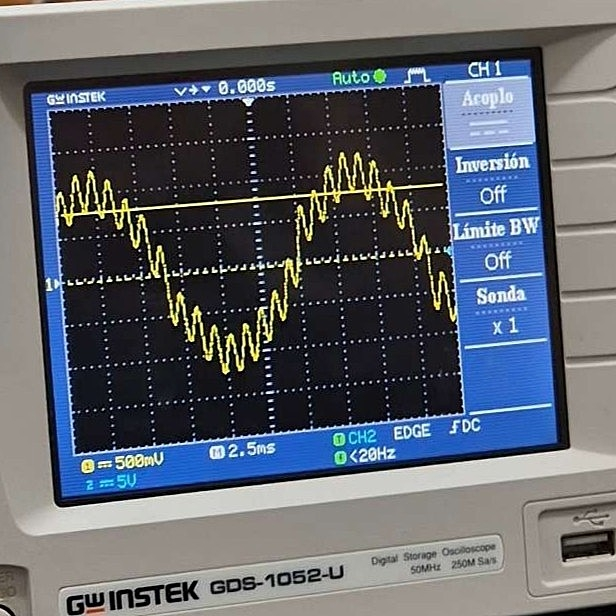
\includegraphics[width=0.35\textwidth]{imagenes/caso3.jpg}
				\caption{Caso 3: Frecuencias distintas amplitudes iguales.}
				\label{fig:caso3}
			\end{figure}
			\item Para el último caso, tanto las frecuencias como las amplitudes fueron distintos, así en el osciloscopio se observó algo muy similar al caso
			anterior, pero en la FFT se observó claramente dos picos con frecuencias distintas y alturas distintas. Observar Figura \ref{fig:caso4}
			\begin{figure}[ht]
				\centering
				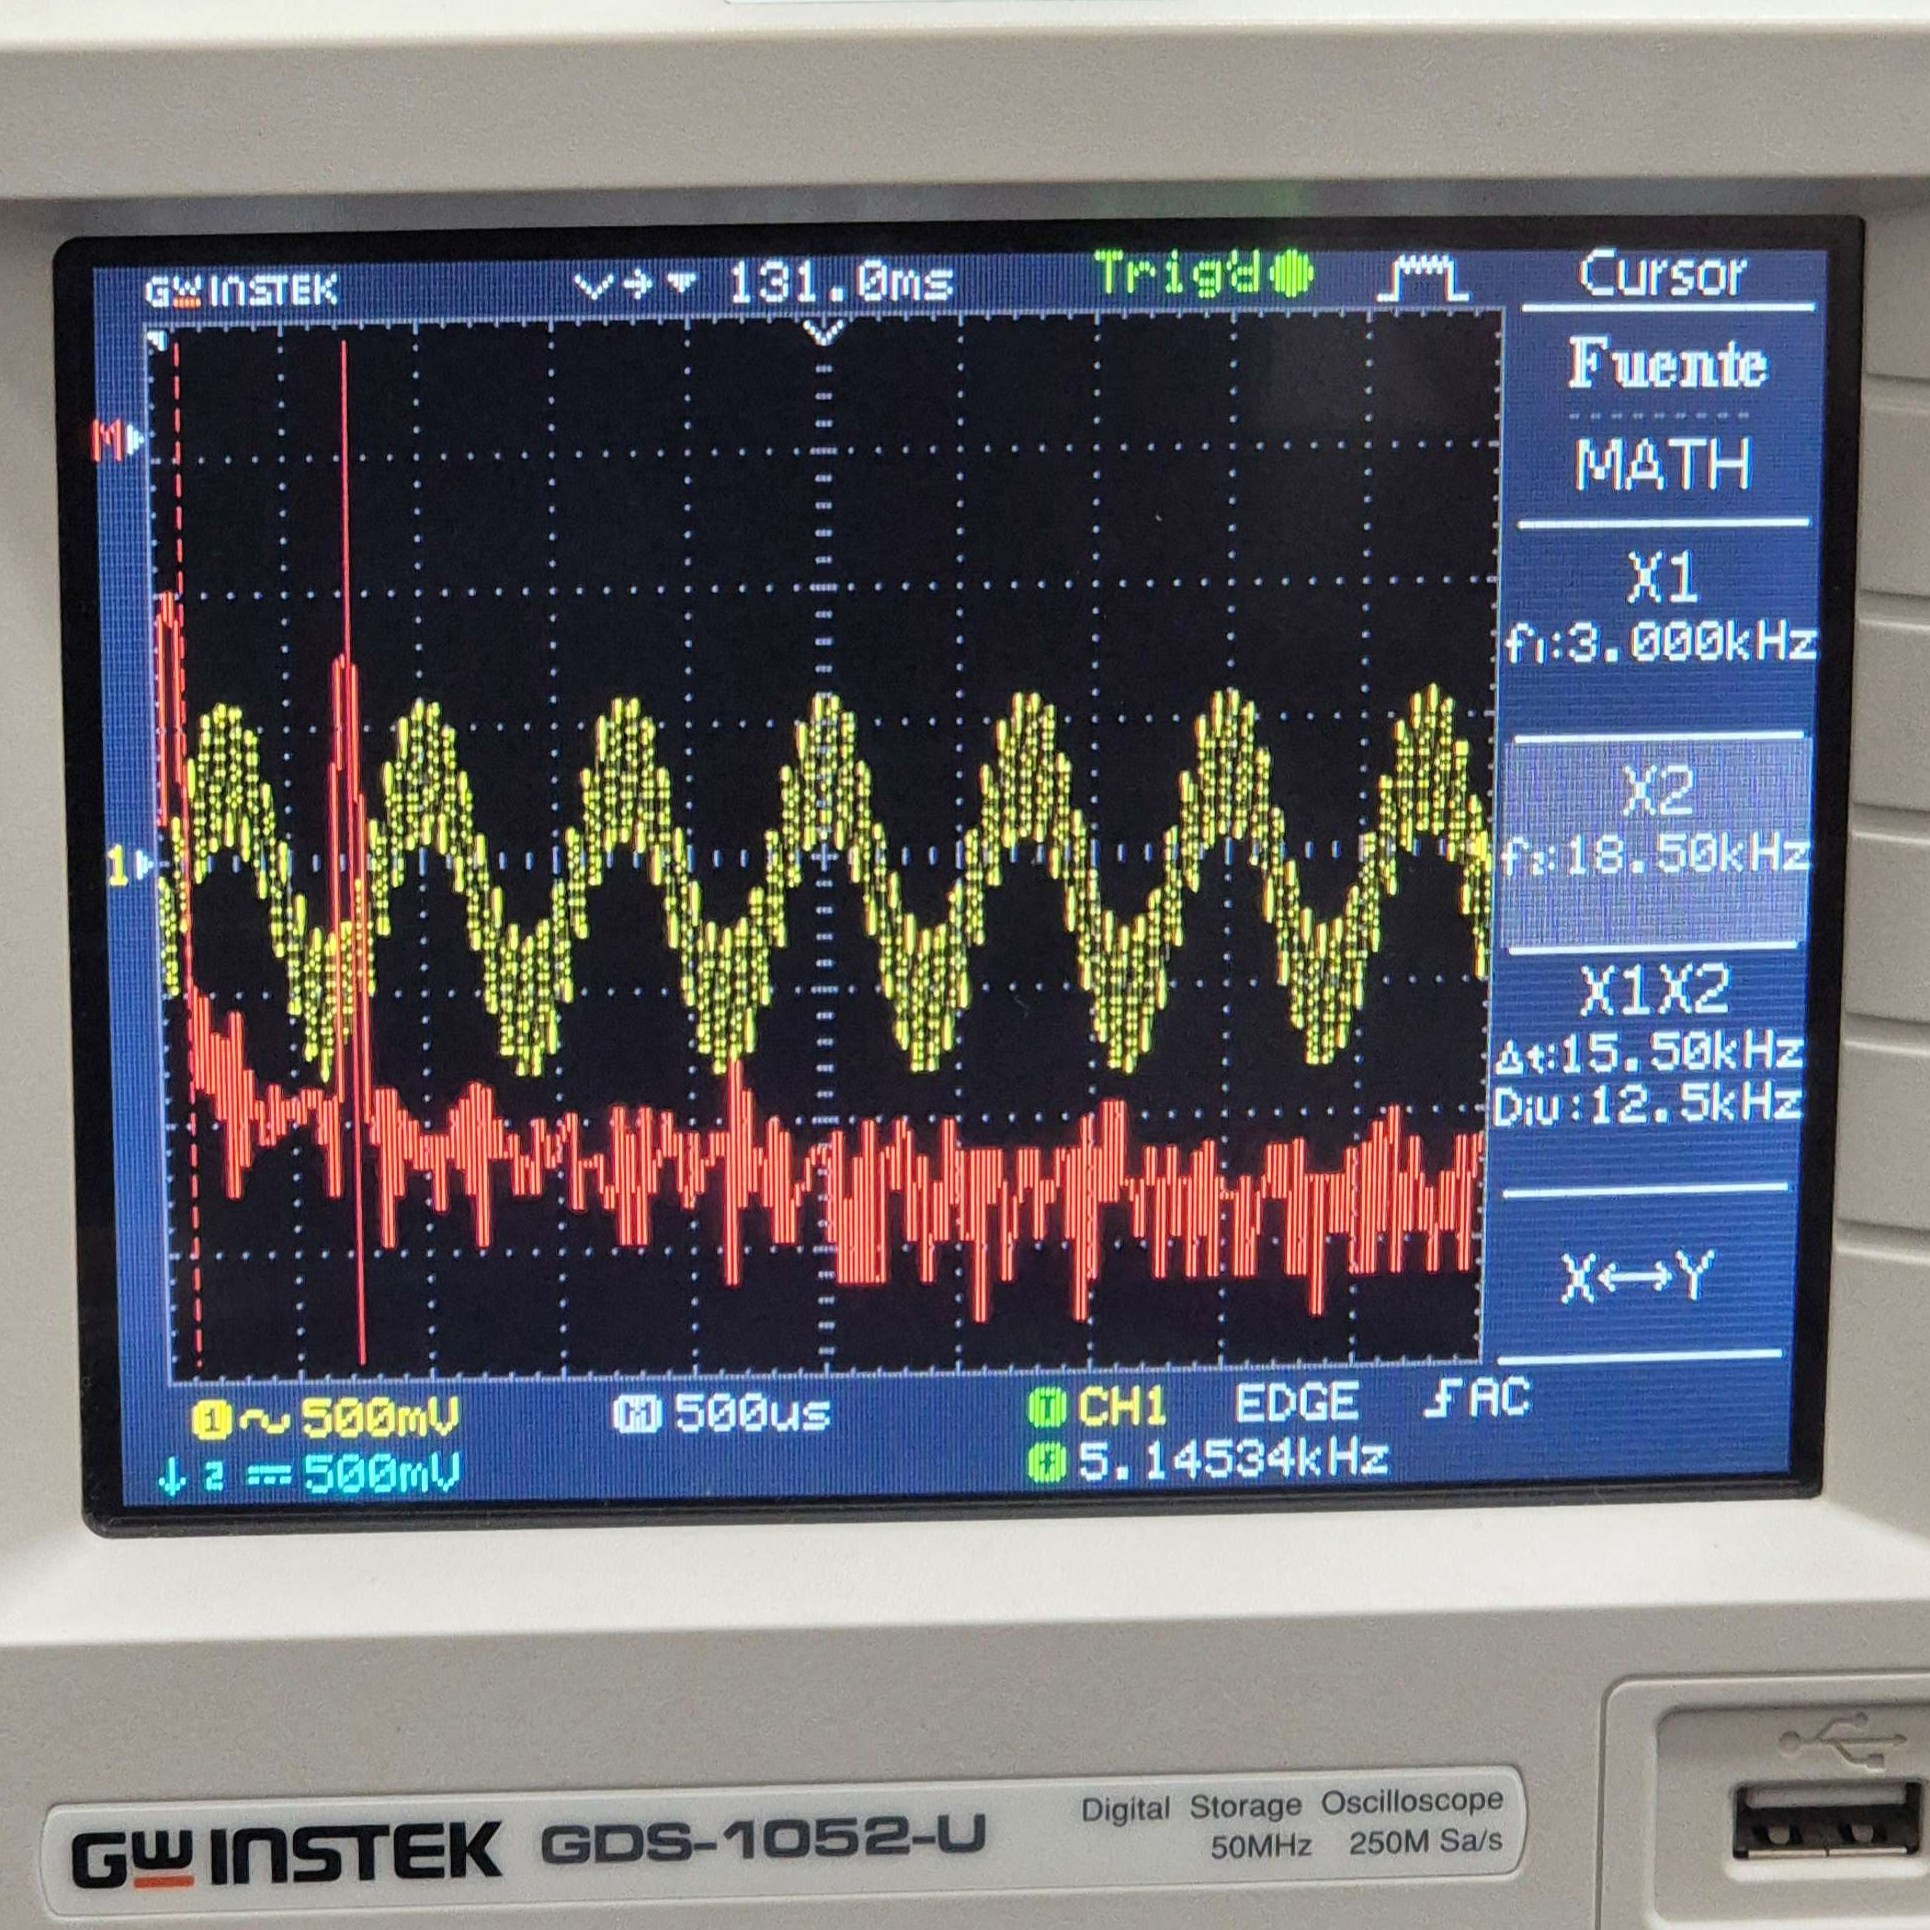
\includegraphics[width=0.35\textwidth]{imagenes/caso4.jpg}
				\caption{Caso 4: Frecuencias y amplitudes distintas.}
				\label{fig:caso4}
			\end{figure}
		\end{itemize}

		\subsection{Barrido y Ancho de Banda}
		Una de las opciones que tiene el Generador del EGOS es el \textbf{Barrido}, en el cual se presentan dos conexiones BNC que, al conectar cada una a
		un canal del Osciloscopio y desplazarlas verticalmente para que no se superpongan, observaremos dos señales muy distinas. En primer lugar, se muestra
		una señal de rampa periódica, y por otro lado, una señal de banda ancha.\\

		Esto es debido a que, como su nombre lo indica, el barrido es en realidad un ``barrido de frecuencias'', por lo que la señal rampa funciona como un
		modulador de frecuencias para la señal de banda ancha tal que la frecuencia aumentará linealmente mientras la rampa sube y cuando esta se reinicie las
		frecuencias también lo harán.\\
		Mediante la FFT se puede visualizar muy bien el \textbf{Ancho de banda}, pues en lugar de solo tener picos como en los anteriores casos, esta vez
		se obtienen muchísimos picos que se ven como una ``montaña'' sólida de frecuencias, es decir, que el ancho de banda es un conjunto de muchas componentes
		frecuenciales.\\
		La forma de medir en el osciloscopio el ancho de banda es, justo donde este alcanza su máximo y se mantiene recto, bajamos unos $3 dB$
		de ambos lados y la resta de estos valores de frecuencias nos da el valor del ancho de banda.\\
		Lo mencionado se puede observar en la Figura \ref{fig:barrido}.

		\begin{figure}
			\centering
			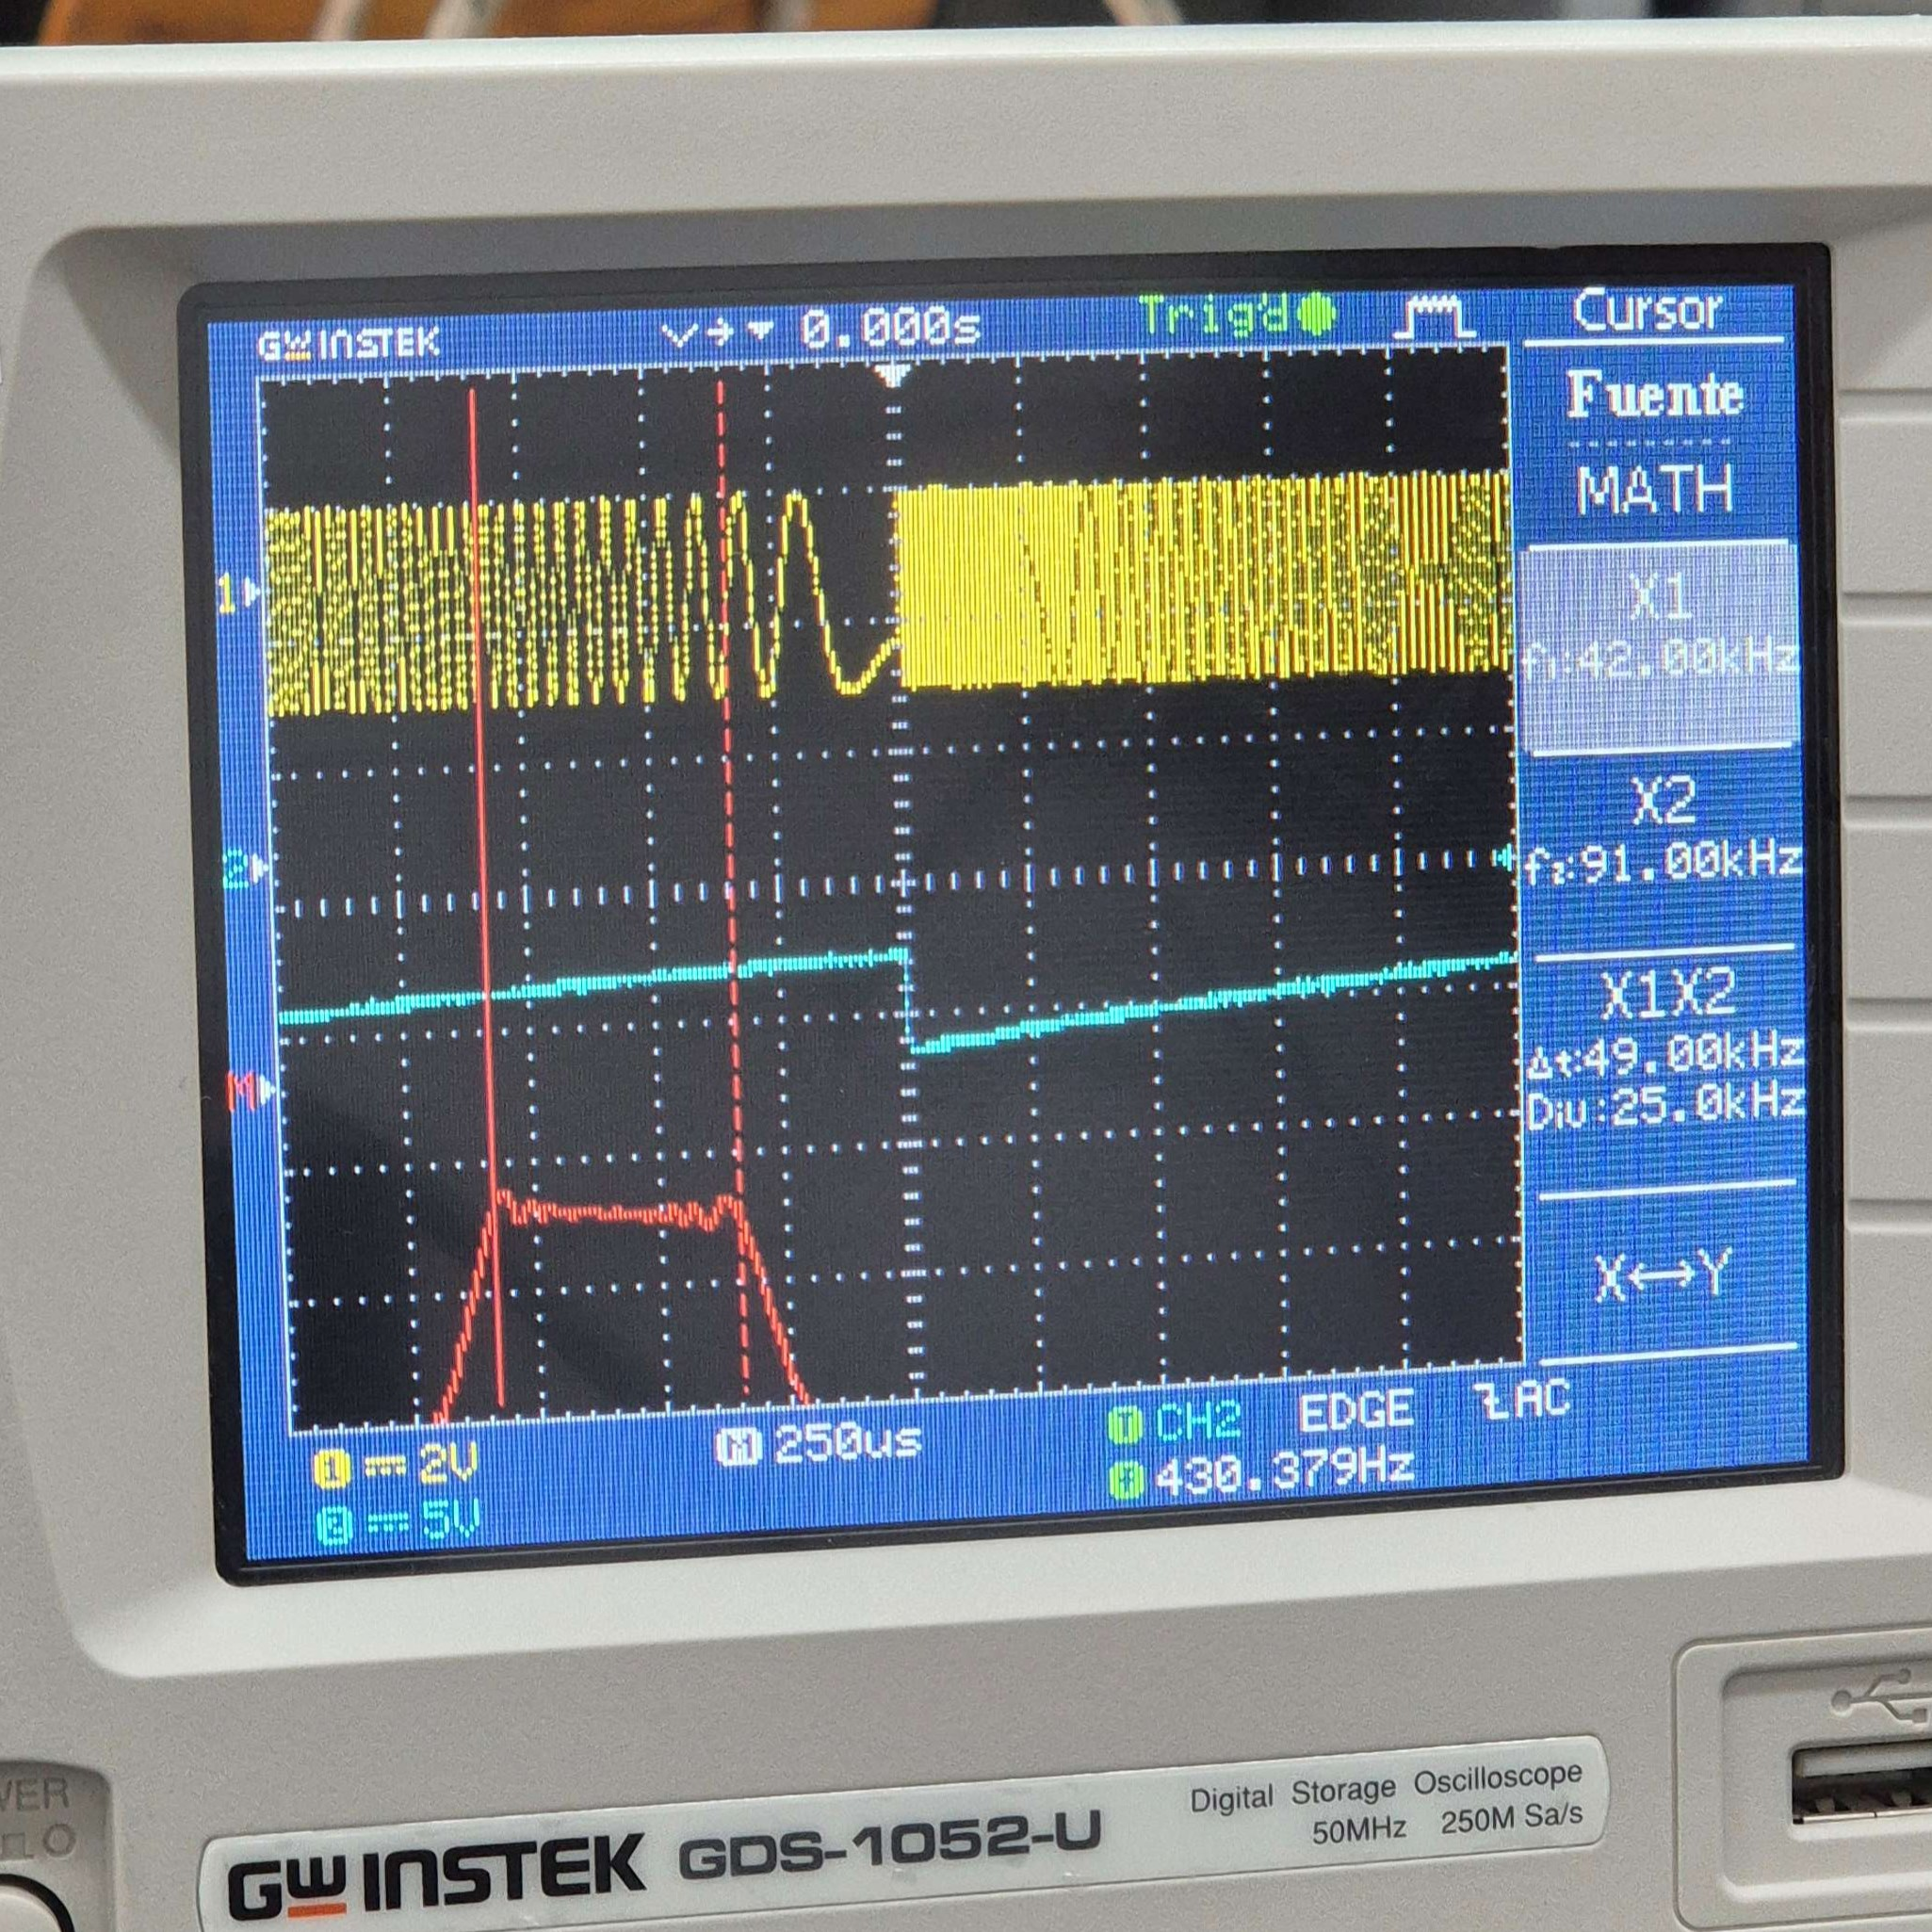
\includegraphics[width=0.35\textwidth]{imagenes/Barrido.jpg}
			\caption{Señal rampa, señal de banda ancha y ancho de banda generadas por el Barrido del EGOS.}
			\label{fig:barrido}
		\end{figure}

		\subsection{Fase y Suma de ondas}
		La otra opcion con la que cuenta el Generador del EGOS es la \textbf{Fase}, que igualmente cuenta con 2 terminales BNC las cuales se conectaron a
		dos canales distintos del Osciloscopio y estas señales se acomodaron de modo que no se encimaran. Además, dentro del menú ``math'' del osciloscopio
		se seleccionó la opción ``CH1 + CH2''. que lo que hace es sumar ambas señales, algo similar a lo que hace el Sumador del EGOS pero de este modo
		nos permite ver ambas señales y su suma por separado.\\

		Ahora, al girar la perilla de Fase lo que se observó, como su nombre lo indica, un desplazamiento en la fase de ambas señales, de modo que en un
		extremo ambas señales estaban desfasadas completamente, dando como resultado una señal casi en cero, mientras que en el otro extremo ambas señales
		estaban completamente en fase, tal que la señal resultante tenía el doble de la amplitud y la misma frecuencia que sus componentes. Las 2 señales
		y su suma en el osciloscopio se pueden ver en la Figura \ref{fig:fase}.\\

		\begin{figure}[ht]
			\centering
			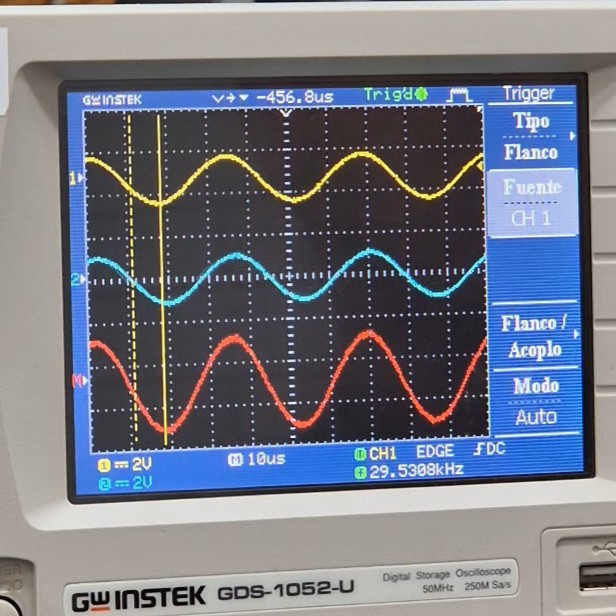
\includegraphics[width=0.35\textwidth]{imagenes/Fase.jpg}
			\caption{Dos señales y su suma vistas en el Osciloscopio.}
			\label{fig:fase}
		\end{figure}

		El Osciloscopio también cuenta con la opción de cambiar los ejes de ``voltaje contra tiempo'' a ``x y'', es decir, ``una señal contra otra señal'',
		en donde se pueden ver las \textbf{Figuras de Lissajous}, las cuales son una relacion de frecuencias y fase entre señales.\\
		Los casos más comunes ocurren cuando tenemos misma frecuencia y fase en ambas señales, por lo que se observa una linea recta inclinada, o cuando
		tenemos misma frecuencia pero en desfase se observan elipses, y si las frecuencias son distintas se forman figuras complejas (lazos) como las
		obtenidas en la Figura \ref{fig:Lissajous}.

		\begin{figure}[ht]
			\centering
			\begin{subfigure}[b]{0.30\columnwidth}
				\centering
				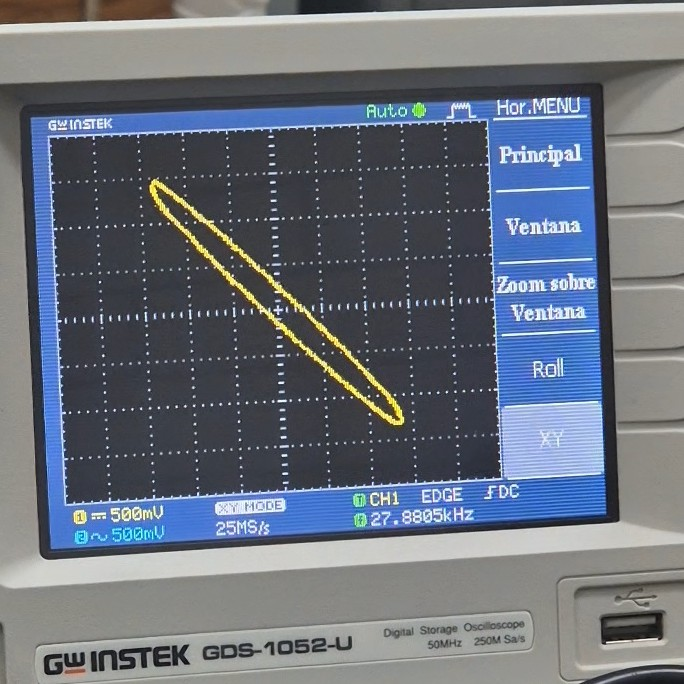
\includegraphics[width=\linewidth, keepaspectratio]{imagenes/Lissajous1.jpg}
			\end{subfigure}
			\hfill
			\begin{subfigure}[b]{0.30\columnwidth}
				\centering
				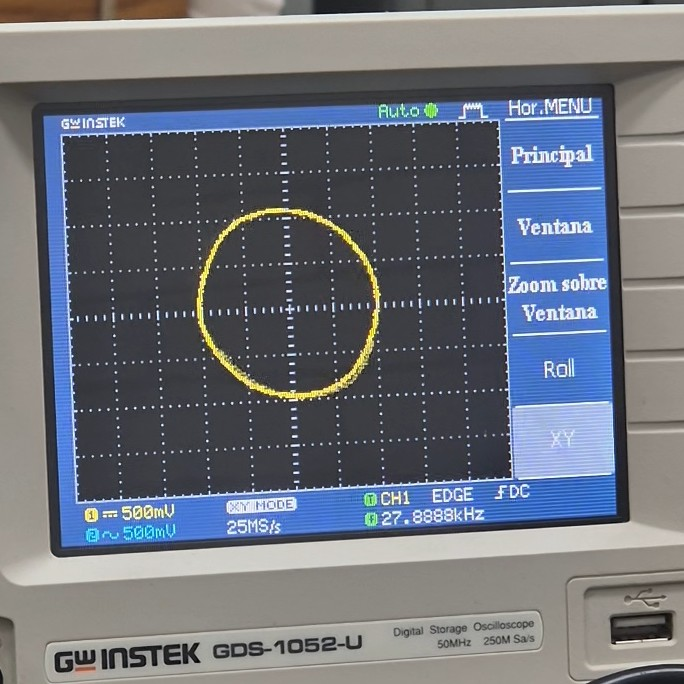
\includegraphics[width=\linewidth, keepaspectratio]{imagenes/Lissajous2.jpg}
			\end{subfigure}
			\hfill
			\begin{subfigure}[b]{0.30\columnwidth}
				\centering
				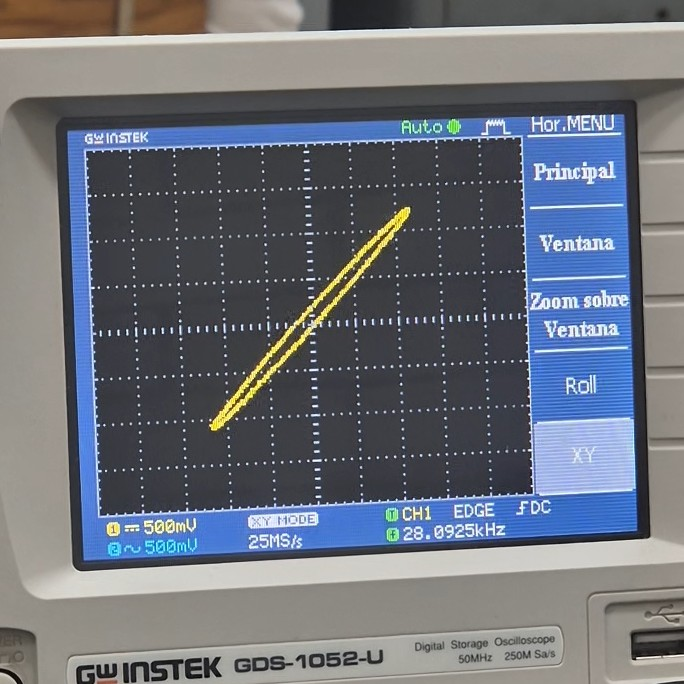
\includegraphics[width=\linewidth, keepaspectratio]{imagenes/Lissajous3.jpg}
			\end{subfigure}
			\caption{Figuras de Lissajous obtenidas con la opcion ``XY'' del osciloscopio al variar la fase con el EGOS.}
			\label{fig:Lissajous}
		\end{figure}
		

	\section{Transformador + Fuente Simétrica}
	Como se mencionó anteriormente, el Transformador es una fuente de voltaje AC mientras que la Fuente Simétrica proporciona un voltaje constante,
	el objetivo de este experimento fue conectar ambos al osciloscopio por un solo canal con ayuda del Sumador del EGOS, sin embargo, buscamos un
	voltaje máximo de $5 V_{PP}$ o $1.75 V_{RMS}$ de modo que se tuvo que armar un \textbf{Divisor de voltaje} para cada instrumento.\\
	
	Para la Fuente Simétrica, la cual proporcionaba $12 V$, elegimos dos resistencias de $1 k\Omega$ y $12 k\Omega$ para el divisor, obteniendo en
	la resistencia de menor valor $0.93 V$ y $0.00 V_{RMS}$. Por otro lado, para el Transformador elegimos resistencias de $1 k\Omega$ y $15 k\Omega$,
	obteniendo en la resistencia de menor valor $0.025 mV$ y $0.83 V_{RMS}$. La señal resultante del osciloscopio fue una suma de una señal DC más
	una señal AC, por lo que, graficamente se visualizó como una señal AC con un desplazamiento de voltaje inicial.

	% \printbibliography

	\onecolumn
	\appendix
    \section{Tablas de datos}
	\label{apx:1}

		\begin{table}[ht]
		\centering
			\begin{tabular}{|c|c|c|}
			\hline
			Forma      & DC [$mV$] & AC [$V_{RMS}$] \\ \hline
			Senoidal   & 7.6 - 9.0 & 3.46           \\ \hline
			Triangular & 1.4 - 2.6 & 3.94           \\ \hline
			Cuadrada   & 0.7 - 3.2 & 4.94           \\ \hline
			\end{tabular}
		\caption{Valores medidos por el multímetro para cada forma de onda.}
		\label{tab:triangular}
		\end{table}
	
\end{document}